\chapter{绪论}\label{DS01}

\section{数据结构与抽象数据类型}\label{DS01-structure}

\par\smallskip
{\fontsize{9.3}{12}\selectfont\setlength{\tabcolsep}{2.5pt}\setlength{\LTleft}{0pt}\setlength{\LTright}{0pt}
\begin{longtable}{@{}>{\raggedright\arraybackslash}p{\dimexpr0.39199\linewidth-2\tabcolsep\relax}>{\raggedright\arraybackslash}p{\dimexpr0.60801\linewidth-2\tabcolsep\relax}@{}}
\toprule
概念 & 定义与判断依据 \\

\midrule\endfirsthead\toprule
概念 & 定义与判断依据 \\

\midrule\endhead\bottomrule\endfoot
数据元素 & 数据处理的基本单位；由若干数据项组成 \\

数据项 & 构成数据元素的不可分割的最小单位 \\

数据对象 & 性质相同的数据元素的集合 \\

逻辑结构 & 元素间的关系：集合、线性、树形、图状 \\

存储结构 & 元素及其关系的机器表示：顺序、链式、索引、散列 \\

数据运算 & 运算的抽象定义及其在具体存储结构上的实现 \\

数据类型 & 值的集合及定义在该集合上的操作 \\

抽象数据类型（ADT） & 数据对象、关系和操作的抽象描述，隐藏具体实现 \\

\end{longtable}}
\par\smallskip

数据结构的三要素为\textbf{逻辑结构、存储结构、数据的运算}。同一逻辑结构可采用不同存储结构；链式存储可表示线性表、树或图。栈、队列属于线性结构，允许的操作位置各有约束。顺序存储以连续位置体现关系，链式存储以链接体现关系。

\begin{figure}[H]
\centering
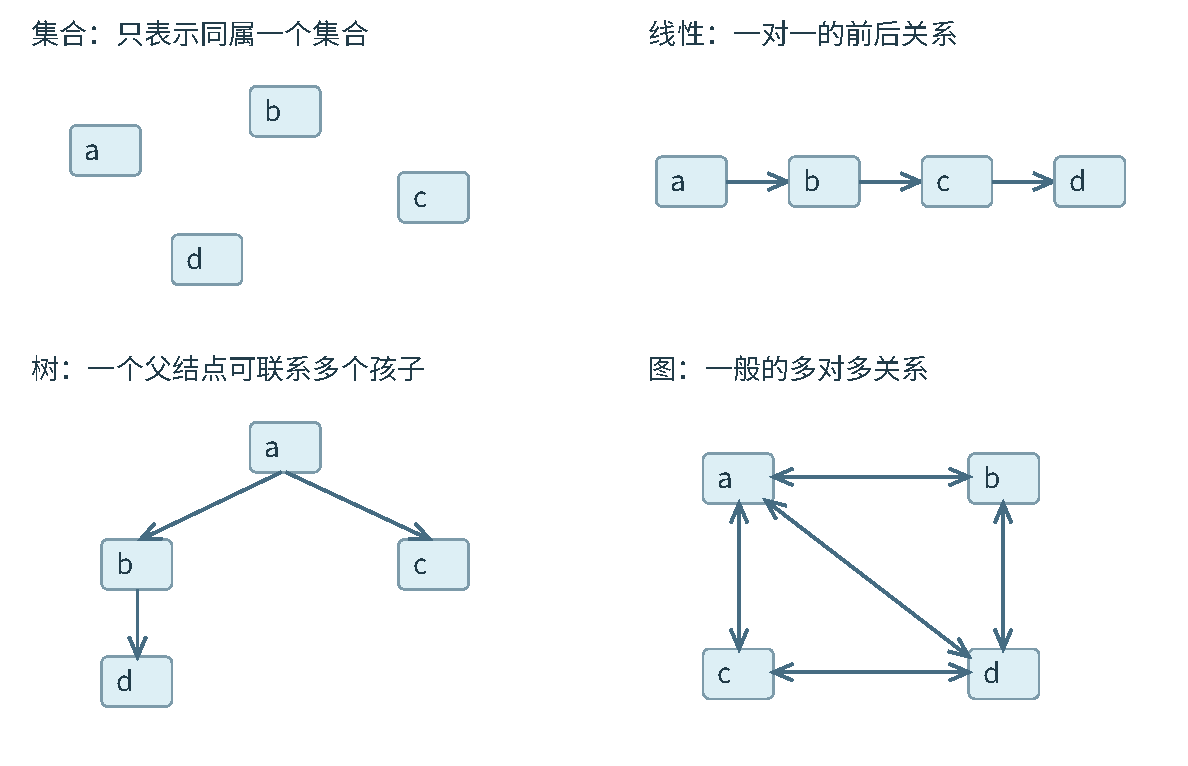
\includegraphics[width=\linewidth,height=108mm,keepaspectratio]{figures/DS01_logical_structures.pdf}
\caption{四类逻辑结构}\label{DS01-logical-figure}
\end{figure}

\par\medskip\Needspace{4\baselineskip}\noindent\hypertarget{DS01-E01}{}\label{DS01-E01}\textbf{例 1-1}\par\nobreak\smallskip

在存储数据时，通常不仅要存储各数据元素的值，还要存储（　）。

A. 数据的操作方法　B. 数据元素的类型　C. 数据元素之间的关系　D. 数据的存取方法

\section{算法特性与正确性}\label{DS01-algorithm}

算法是求解一类问题的有限操作序列，具有\textbf{有穷性、确定性、可行性、输入、输出}五项特性：对每次合法输入，有限步结束；每步含义明确且能在有限时间内执行；输入可为零个或多个，输出至少一个。返回值或修改后的状态均可作为输出。

算法设计还评价正确性、可读性、健壮性及时间、空间效率。可行性只要求操作可执行；时空效率取决于操作次数和所需资源。

循环正确性按\textbf{初始化---保持---终止}证明循环不变式，并说明循环确实接近终止边界。最大值扫描要求非空数组；若接受空数组，应返回失败。

\par\smallskip\noindent\begin{minipage}{\linewidth}
\begin{codeblock}[language={C++}]
bool maximum(int a[], int n, int &answer) {
    if (n <= 0) return false;
    int best = a[0];
    for (int i = 1; i < n; ++i)
        if (a[i] > best) best = a[i];
    answer = best;
    return true;
}
\end{codeblock}
\end{minipage}\par\smallskip

第\(i\)轮前，\texttt{best}为\texttt{a[\allowbreak{}0.\allowbreak{}.\allowbreak{}i-1]\allowbreak{}}的最大值；更新后扩展到\texttt{a[\allowbreak{}0.\allowbreak{}.\allowbreak{}i]\allowbreak{}}。终止时覆盖全部元素。合法输入做\(n-1\)次元素比较，时间\(\Theta(n)\)、辅助空间\(\Theta(1)\)。比较记录中的关键字时，移动操作须携带整条记录的各数据项。

\section{渐近时间复杂度}\label{DS01-time}

选择基本操作，计算其执行次数\(T(n)\)，再提取增长阶。单位成本模型将定长比较、赋值、数组访问看作常数时间；大整数、外存访问等需另定成本模型。

\begin{itemize}
\tightlist
\item
  \(O(f(n))\)：渐近上界；\(\Omega(f(n))\)：渐近下界；\(\Theta(f(n))\)：同阶的上下界。
\item
  顺序执行：相加后取主阶；重复或嵌套：按实际每轮次数求和。
\item
  常数因子与低次项不改变增长阶；固定底数的对数只相差常数因子。
\end{itemize}

按渐近增长率排序，\(c>1\)为常数，对数底数为固定大于1的常数：

\[1 < \log n < n < n\log n < n^2 < n^3 < c^n < n! < n^n.\]

\par\smallskip
{\fontsize{9.3}{12}\selectfont\setlength{\tabcolsep}{2.5pt}\setlength{\LTleft}{0pt}\setlength{\LTright}{0pt}
\begin{longtable}{@{}>{\raggedright\arraybackslash}p{\dimexpr0.40979\linewidth-2\tabcolsep\relax}>{\raggedright\arraybackslash}p{\dimexpr0.36429\linewidth-2\tabcolsep\relax}>{\raggedright\arraybackslash}p{\dimexpr0.22592\linewidth-2\tabcolsep\relax}@{}}
\toprule
代码特征 & 次数关系 & 紧数量级 \\

\midrule\endfirsthead\toprule
代码特征 & 次数关系 & 紧数量级 \\

\midrule\endhead\bottomrule\endfoot
\texttt{i++}到\(n\) & \(n\) & \(\Theta(n)\) \\

\texttt{i*=2}或整数\texttt{i/=2} & 次数与\(\log_2n\)同阶 & \(\Theta(\log n)\) \\

第\(i\)轮执行\(i\)次，\(i=1..n\) & \(\sum_{i=1}^n i=n(n+1)/2\) & \(\Theta(n^2)\) \\

第\(i\)轮执行\(2^i\)次，共至\(\log_2n\)轮 & 等比和 & \(\Theta(n)\) \\

\(T(n)=T(n-1)+\Theta(1)\) & 线性层数 & \(\Theta(n)\) \\

\(T(n)=2T(n/2)+\Theta(n)\) & 每层线性，约\(\log_2n\)层 & \(\Theta(n\log n)\) \\

\end{longtable}}
\par\smallskip

\par\medskip\Needspace{4\baselineskip}\noindent\hypertarget{DS01-E02}{}\label{DS01-E02}\textbf{例 1-2}\par\nobreak\smallskip

下列函数的时间复杂度是（　）。

\par\smallskip\noindent\begin{minipage}{\linewidth}
\begin{codeblock}[language={C}]
int func(int n) {
    int i=0, sum=0;
    while (sum<n) sum += ++i;
    return i;
}
\end{codeblock}
\end{minipage}\par\smallskip

A. \(O(\log n)\)　B. \(O(n^{1/2})\)　C. \(O(n)\)　D. \(O(n\log n)\)

\par\medskip\Needspace{4\baselineskip}\noindent\hypertarget{DS01-E03}{}\label{DS01-E03}\textbf{例 1-3}\par\nobreak\smallskip

下列程序段的时间复杂度是（　）。

\par\smallskip\noindent\begin{minipage}{\linewidth}
\begin{codeblock}[language={C}]
int sum=0;
for (int i=1; i<n; i*=2)
    for (int j=0; j<i; j++)
        sum++;
\end{codeblock}
\end{minipage}\par\smallskip

A. \(O(\log n)\)　B. \(O(n)\)　C. \(O(n\log n)\)　D. \(O(n^2)\)

\par\medskip\Needspace{4\baselineskip}\noindent\hypertarget{DS01-E04}{}\label{DS01-E04}\textbf{例 1-4}\par\nobreak\smallskip

设n是描述问题规模的非负整数，程序段\texttt{x=\allowbreak{}0;\allowbreak{} while(\allowbreak{}n>\allowbreak{}=\allowbreak{}(\allowbreak{}x+\allowbreak{}1)\allowbreak{}*\allowbreak{}(\allowbreak{}x+\allowbreak{}1)\allowbreak{})\allowbreak{} x=\allowbreak{}x+\allowbreak{}1;\allowbreak{}}的时间复杂度是（　）。

A. \(O(\log n)\)　B. \(O(n^{1/2})\)　C. \(O(n)\)　D. \(O(n^2)\)

\textbf{最好、最坏、平均}均针对相同规模的输入：分别取最少、最多、按给定概率分布加权的工作量。平均值需要概率模型。等概率且保证成功的顺序查找平均比较\((n+1)/2\)次；包含失败时另加失败概率与代价。\(O/\Omega/\Theta\)与最好/最坏属于两套不同分类。

\section{辅助空间与递归栈}\label{DS01-space}

辅助空间统计同一时刻存活的额外状态，通常排除输入，输出区按题意处理。顺序复用的空间取峰值，同时保留的空间相加。原地算法通常要求常数辅助空间。

\par\smallskip
{\fontsize{9.3}{12}\selectfont\setlength{\tabcolsep}{2.5pt}\setlength{\LTleft}{0pt}\setlength{\LTright}{0pt}
\begin{longtable}{@{}>{\raggedright\arraybackslash}p{\dimexpr0.59573\linewidth-2\tabcolsep\relax}>{\raggedright\arraybackslash}p{\dimexpr0.40427\linewidth-2\tabcolsep\relax}@{}}
\toprule
同时活跃状态 & 峰值辅助空间 \\

\midrule\endfirsthead\toprule
同时活跃状态 & 峰值辅助空间 \\

\midrule\endhead\bottomrule\endfoot
常数个变量反复执行\(n\)轮 & \(\Theta(1)\) \\

每轮复用长度\(n\)的数组，共\(n\)轮 & \(\Theta(n)\) \\

递归深度\(n\)，每层常数空间 & \(\Theta(n)\) \\

一条调用链各层保留\(n,n-1,\ldots,1\)个单元 & \(\Theta(n^2)\) \\

一条调用链各层保留\(n,n/2,n/4,\ldots\)个单元 & \(\Theta(n)\) \\

二叉树递归遍历，树高\(h\) & \(O(h)\)；总时间\(\Theta(n)\) \\

\end{longtable}}
\par\smallskip

递归树的调用总数决定总工作量，最长未返回调用链决定栈深。快速排序的普通递归实现在平均情况下需\(O(\log n)\)栈空间，最坏需\(O(n)\)。
